\documentclass{mnnit}
\usepackage{graphicx}
\usepackage{url}
\begin{document}
\title{ALEC - (Artificial Linguistic Enquiry Chatbot)}
\author{Aishwarya Sadana(2017CA12)\\Aditya Bhawsar(2017CA59)\\Mansi Sharma(2017CA79)\\Pavan Chandravanshi(2017CA56)}
\supervisor{Dr. Anoj Kumar}
\specialization{Computer Science \& Engineering}
\beforepreface
\prefacesection{Preface}
A \textbf{Chatbot} is a computer program or an artificial intelligence which
conducts a conversation via auditory or textual methods.A Chatbot for any website
helps to find out the queries through chat. We can get the answers instantly
without searching it in the whole website and if the query is not available it
asks to submit the query later the admin will add the answers for it. It is an
advanced and promising expression of interaction batween human aad machine. ALEC
that we made, using PHP, HTML, CSS, JavaScript and Python, caters all of these
requirements and helps the students to find answers to their queries instantly.\\

\prefacesection{Acknowledgements}
It is obvious that the development of this project needed the support of many people. We would like to
express my deepest appreciation to all those who provided us the possibility to complete this project.
First of all, we would like to thank our Head of Department, \textbf{Prof. A. K. Singh}, to give us the opportunity
to take up this project.
\vspace{10pt}
\newline
Special thanks goes to our project mentor,\textbf{Dr. Anoj Kumar}, under whose guidance we have developed
this project. We are indebted to him for his constant support and encouragement to bring this project
in its present form. With his able guidance and suggestions only we could develop ALEC.
\vspace{10pt}
\newline
Finally, we would also like to raise a vote of thanks to our classmates who have supported and
motivated us in every possible way they could. Their reviews mattered a lot during the development of
this project.
\afterpreface

\chapter{Introduction}
A.L.E.C. stands for ``Artificial Linguistic Enquiry Chatbot''. It will act as a
one place solution to all the queries asked by the students. It will help the
students to get the desired information at the right time. It will be like a virtual assistant to which we can ask questions and get instant answers.
\section{Problem Statement}
The website of Computer Science and engineering Department contains all the
information required by students. But it is very difficult to search for the
information on the site without any prior knowledge of where it could be found.
Students need to enquire information about the department, courses, subjects,
past projects, etc. They need to search through the website to look for answers.
It can be time consuming or sometime information is not present on the website.
Students need to manually visit to the college to get their queries answered by
the college help desk. This process consumes lot of time as well as money as the
customer needed to visit college if its miles away from home. Also, this process
may lead to communication gap between student and college.

\section{Objective}
To create a Chat Bot for the Computer Science and Engineering Department which
will help student's to get answer to their query, immediately and efficiently.

\section{About The Project}
Chat bots typically provide a text-based user interface, allowing the user to
type commands and receive text as well as text to speech response. Chat bots are
usually stateful services, remembering previous commands in order to provide
functionality. When chat bot technology is integrated with popular web services
it can be utilized securely by an even larger audience.
\vspace{10pt}
\newline
A.L.E.C. is built with python's \textbf{ChatterBot} library using machine
learning algorithms that analyzes user's queries, understand user's message and
provide right answer. This System will be a web application which provides answer
to the query of the student very effectively. Students just have to put their
query to the bot which is used for chatting. The system will use the artificial
intelligence algorithms to give appropriate answers to the user. The student will
not have to go to the college for enquiring something. Student can use the chat
bot to get the answers to their queries at any point of time. This system may
help students to stay updated with the college activities.
\vspace{10pt}
\newline
This is an advanced PHP,HTML, CSS, JavaStript and Python Chatbot system that
will allow you to chat with the machine and get a detailed information in return.
It includes:

\begin{itemize}
	\item Chat view.
	\item Active communication method
	\item Notice Board for CSED
\end{itemize}


\section{Motivation}
In this fast growing technical world being student of a technical institution we
still have to find answer to our query manually by going to the dapartment, which
makes us old school and can cost us our time and money too. We want to develop a
web application which can give us answers to our queries of any type at any time
in minimum cost. We sometimes pass our time by chatting with different ChatBot
available on internet, so to make one of them was indeed an interesting idea. For
learning aspect, we wanted to work on a full web-application and apply all the
concepts they we have learned in the past years.

\section{Related Work}
Since currently we do not have any Chatbot for CSED, we had to look for other
sources for related work. \textbf{Cleverbot[2], Disha[3], etc.} are some
frequently used chatbots but none of them can fulfill our requirement.

\chapter{Design Methodology Used}
We used the basic Waterfall Model to Develop our project.\\
In waterfall model we follow the following steps to develop the project
\begin{enumerate}
\item Gather information
\item Design
\item Implement
\item Perform testing
\item Maintenance
\end{enumerate}
This model is very simple to understand and implement. However, due to its\\
simplicity, this model is only useful for a limited type of projects.\\\\
Following are the reasons why we choose this model:
\begin{enumerate}
\item Our requirements were rigidly defined from the very beginning.
\item The technology that we were going to use was very well defined.
\item Each phase of the project was clearly defined.
\end{enumerate}


\chapter{Proposed Work}
The system that we are planning to build should support the following basic functionality:

\begin{itemize}
	\item Provides user friendly chat view.
	\item Provides reference links.
	\item Provides tucked information.
	\item Live notice board and announcements.
    \item Admin can manage unanswered questions.
	\item User can submit the queries.
\end{itemize}


\section{Functional and Non-Functional Requirements}
\subsection{Functional Requirements}
   A.L.E.C must support the following features:

\begin{itemize}
	\item The admin can manage unanswered queries and can add it in database if required.
	\item The chatbot should be responsive to users.
	\item Chatbot extracts keyword from the query and provide answers based on it.
	\item Only authorized users can upload notices to notice board.
\end{itemize}
\subsection{Non-Functional Requirements}
\begin{itemize}
	\item The chatbot should be designed in such a way that it should be easy for others to maintain and add new features.
	\item The chatbot should be visually appealing.
	\item The web-app should support web page caching to reduce the response time.
	\item All the functionality of the web-site should be easily testable using automated Unit Tests.
\end{itemize}

\chapter{Design}
\section{Data Flow Diagrams}
\subsection{Level 0}
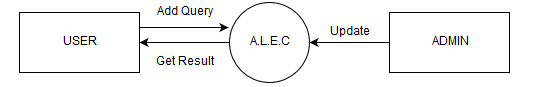
\includegraphics[width=\textwidth]{images/l1.PNG}
\subsection{Level 1}
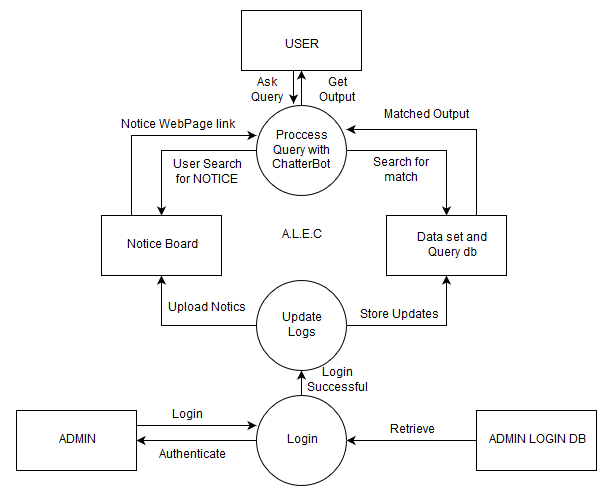
\includegraphics[width=\textwidth, height=200pt]{images/l2.PNG}
\subsection{Level 2}
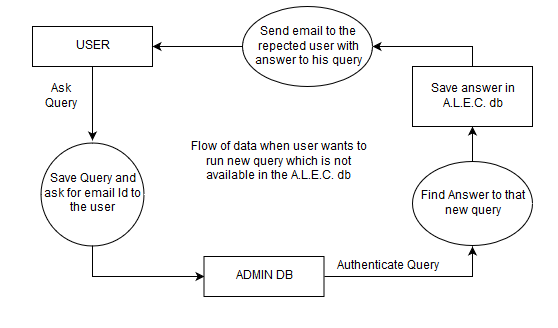
\includegraphics[width=\textwidth, height=200pt]{images/l3.PNG}
\section{Use Case Diagram}
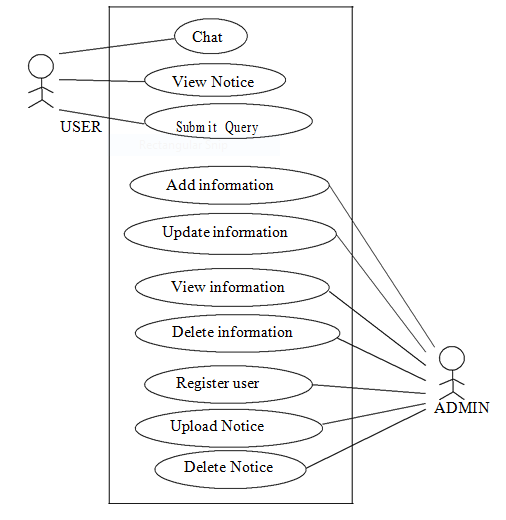
\includegraphics[width=\textwidth, height=300pt]{images/u1.png}



\chapter{Implementation}

\section{Module Details}
A Chatbot have limited number of modules due to its simple and effective functions.  We have divided A.L.E.C. into three modules admin, user and notice board.  These modules are created simultaneously to cater to the needs of students of CSED.
\subsection{Admin}
\begin{itemize}
    \item View information
    \item Update information
    \item Add information
    \item Delete information
    \item Register user to upload notice
    \item Upload notice
    \item Delete notice
\end{itemize}
\subsection{User}
\begin{itemize}
    \item Ask Query
    \item Submit Query
    \item View Notice
\end{itemize}
\subsection{Notice Board}
This module is defined for displaying the important notices issued by the department.  Students can view the notice board by just typing ‘Notice’ in the chatbot.

\section{Corpus Data sets}
Corpus is a large collection of texts.  It is a body of written or spoken material upon which a linguistic analysis is based.  A.L.E.C uses .yml(extension) text files for data sets.  Like,\\
{\textbf{-- --} Good morning! How are you doing?}\\
{\textbf{  --}I am doing very well, thank you for asking.}\\
{\textbf{-- --}You’re welcome.}\\
{\textbf{ --}Do you like hats?}


\section{Python Socket Server}
SimpleWebSocketServer, this asynchronous WebSocket handler create connection with server and client and send data frame to the client.  This library have various functions to facilitate user with packet transferring.  If data is a unicode object then the frame is sent as Text.  If the data is abytearray object then the frame is sent as Binary.

\chapter{Technology and Tools Used}
\section{Python}
Python is an interpreted, object-oriented, high-level programming language with dynamic semantics.  Its high-level built in data structures, combined with dynamic typing and dynamic binding, make it very attractive for Rapid Application Development, as well as for use as a scripting of glue language to connect existing components together.  Large set of available library makes it useful for ALEC.
\section{PHP}
PHP (recursive acronym for PHP: Hypertext Preprocessor) is a widely-used open source general-purpose scripting language that is especially suited for web developmmnt and can be embedded into HTML.
\section{HTML and CSS}
HTML(Hypertext Markup Language) and CSS(Cascading Style Sheets) are two of the core technologies for building Web pages.  HTML provides the structure of the page, CSS the (visual and aural)layout, for a variety of devices.  Along with graphics and scripting, HTML and CSS are the basis of building Web pages and Web Applications.
\section{JavaScript}
JavaScript often abbreviated as "JS", is a high-level, dynamic, untyped, and interpreted run-time language.  In has been standardized in the ECMA Script language specification.  Alongside HTML and CSS, JavaScript is one of the three core technologies of World Wide Web content production; the majority of websites employ it, and all modern Web browsers support it without the need for plugins.  JavaScript is prototype-based with first-class functions, making it multi-paradigm language, supporting object-oriented, imperative, and functional programming styles.  It has an API for working with text, arrays, dates and regular expressions, but does not include any I/O, such as networking, storage, or graphics facilities, relying for these upon the host environment in which it is embedded.
\section{Natural Language ToolKit (NLTK)}
The Natural Language Toolkit (NLTK) is a platform used for building Python programs that work with human language data for applying statistical natural language processing (NLP). It contains text processing libraries for tokenization, parsing, classification, stemming, tagging and semantic reasoning.  It also includes graphical demonstrations and sample data sets as well as accompanied by a cook book and a book which explains the principles behind the underlying language processing tasks that NLTK supports.
\section{ChatterBot Library}
ChatterBot is a Python library that makes it easy to generate automated responses to a user's input.  ChatterBot uses a selection of machine learning algorithms to produce different types of responses.  This makes it easy for developers to create chat bots and automate conversations with users.
\section{MySQL with phpmyadmin}
MySQL is an Oracle-backed open source relational database management system(RDBMS) based on Structured Query Language (SQL). phpMyAdmin is a free software tool written in PHP,intended to handle the administration of MySQL over the Web.  phpMyAdmin supports a wide range of operations on MySQL.
\section{XAMPP}
XAMPP is a free and open-source cross-platform web server solution stackpackage developed by Apache Friends, consisting mainly of the Apache HTTP server, MariaDB database and interpreters for scripts written in the PHP. Since most actual web server deployment use the same component as XAMPP, it makes transitioning from a local test server to a live server possible.

\chapter{Software/Hardware Requirements}
\section{Software Requirements}
\begin{itemize}
	\item Python
    \item Xampp Server
\end{itemize}
\section{System Requirements}
\begin{itemize}
	\item Intel Core (or Dual Core 2GHz) or equal AMD CPU.
	\item 2GB RAM or Above
	\item 40GB of Free HDD Space
\end{itemize}


\chapter{Testing}
\section{Functional Tests}
Since not everything gets covered in Unit Tests, we performed manual functional tests ta make sure that the basic functionalities do not have a bug.  Some of the features that we have tested are:
\begin{itemize}
	\item Accessing all the information on the site (Answers, Results and more).
	\item Multiple tabs working simultaneously without affecting each other.
	\item Adding/Deleting notice for authorised person and admin.
	\item Viewing the Web-App on multiple size windows so that we are sure it is completely responsive.
	\item Trying to access modification rights without Admin Access.
\end{itemize}


\chapter{Experimental Results}
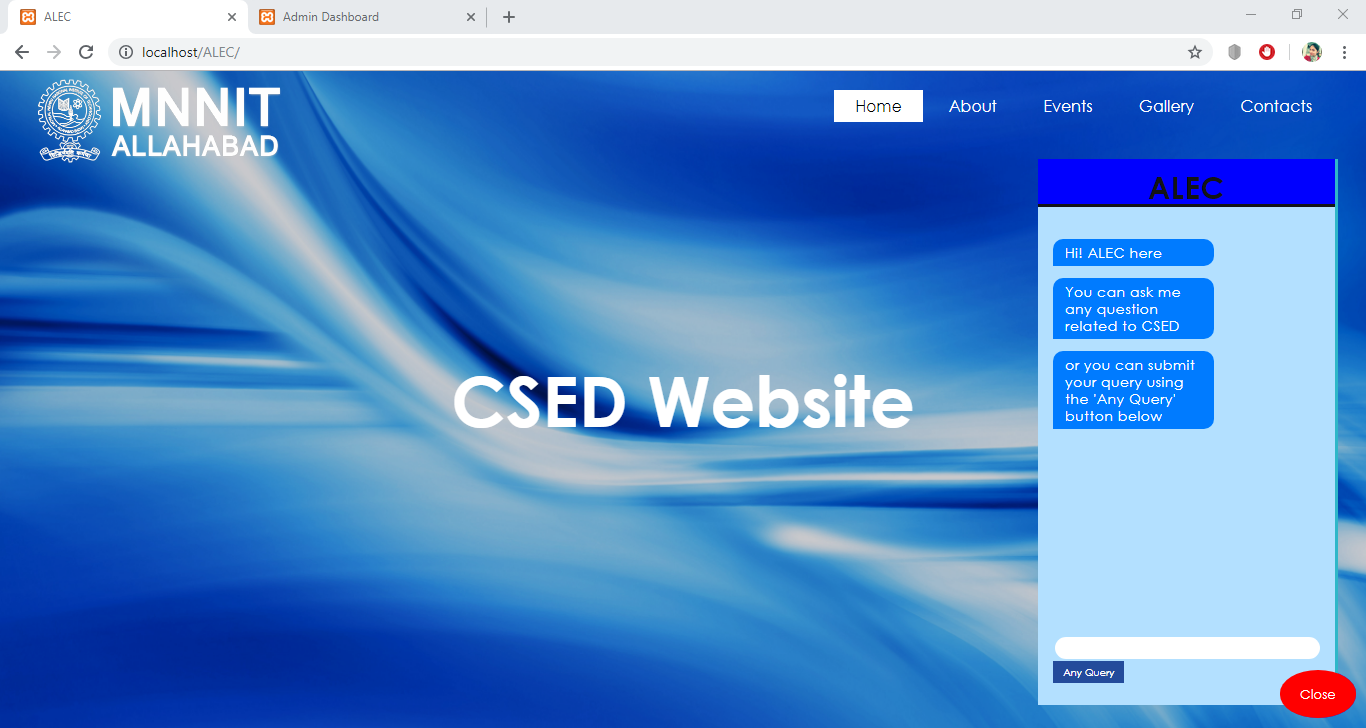
\includegraphics[width=\textwidth]{images/s1.png}
\begin{center}
Fig 9.1: \emph{Initial view of chatbot}
\end{center}
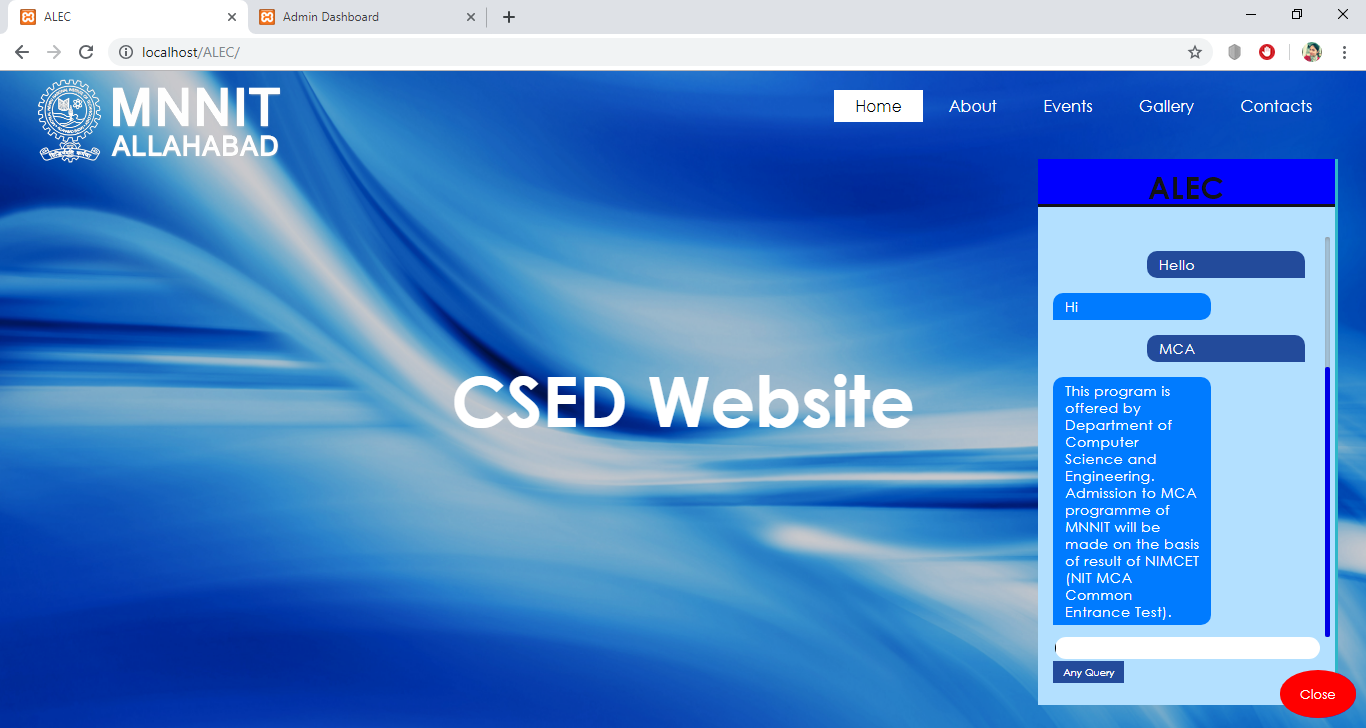
\includegraphics[width=\textwidth]{images/s2.png}
\begin{center}
Fig 9.2: \emph{Reply for MCA given by chatbot}
\end{center}
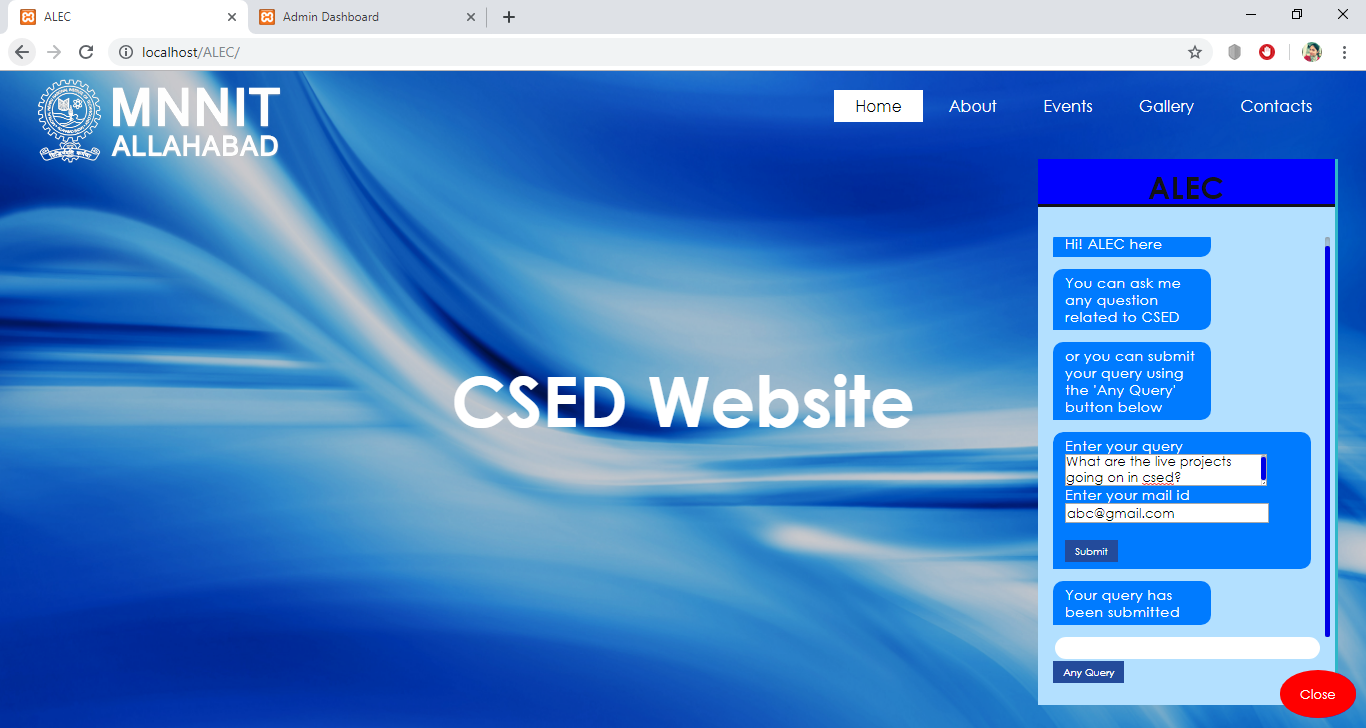
\includegraphics[width=\textwidth]{images/s3.png}
\begin{center}
Fig 9.3: \emph{User submitting query}
\end{center}
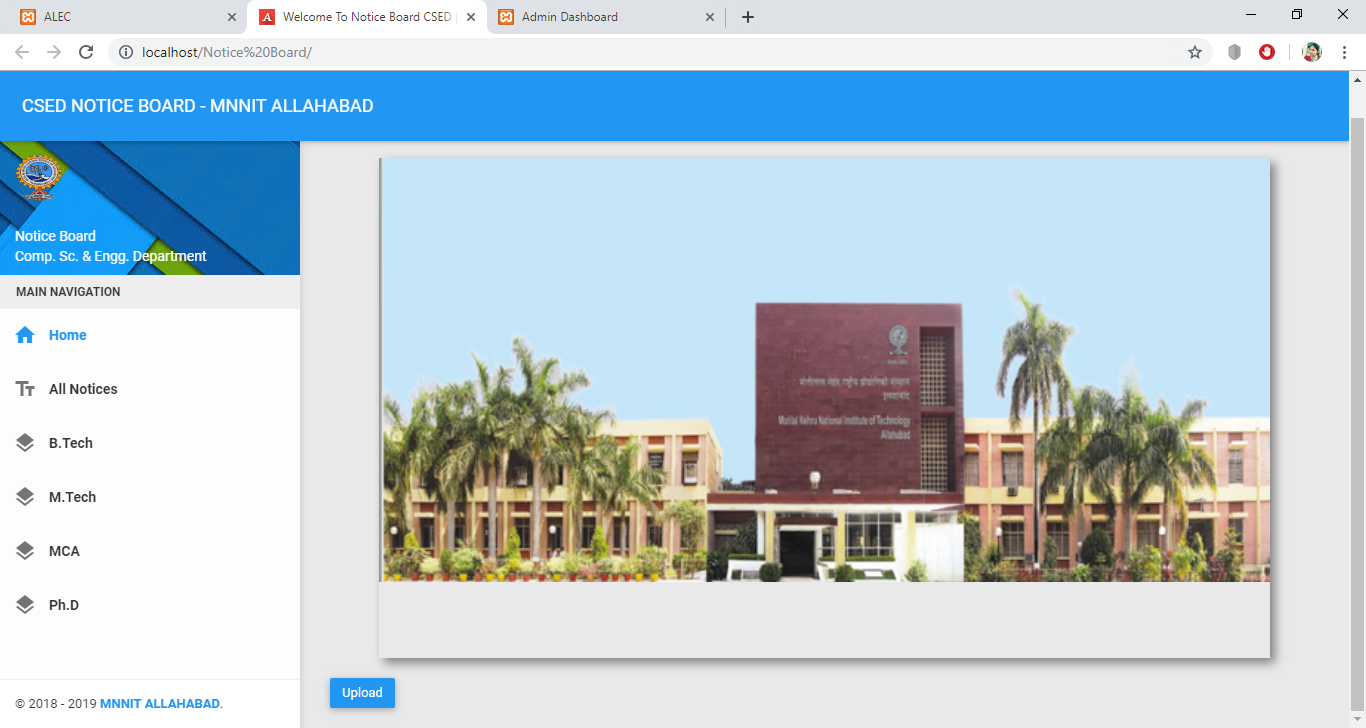
\includegraphics[width=\textwidth]{images/s4.png}
\begin{center}
Fig 9.4: \emph{Notice Board}
\end{center}
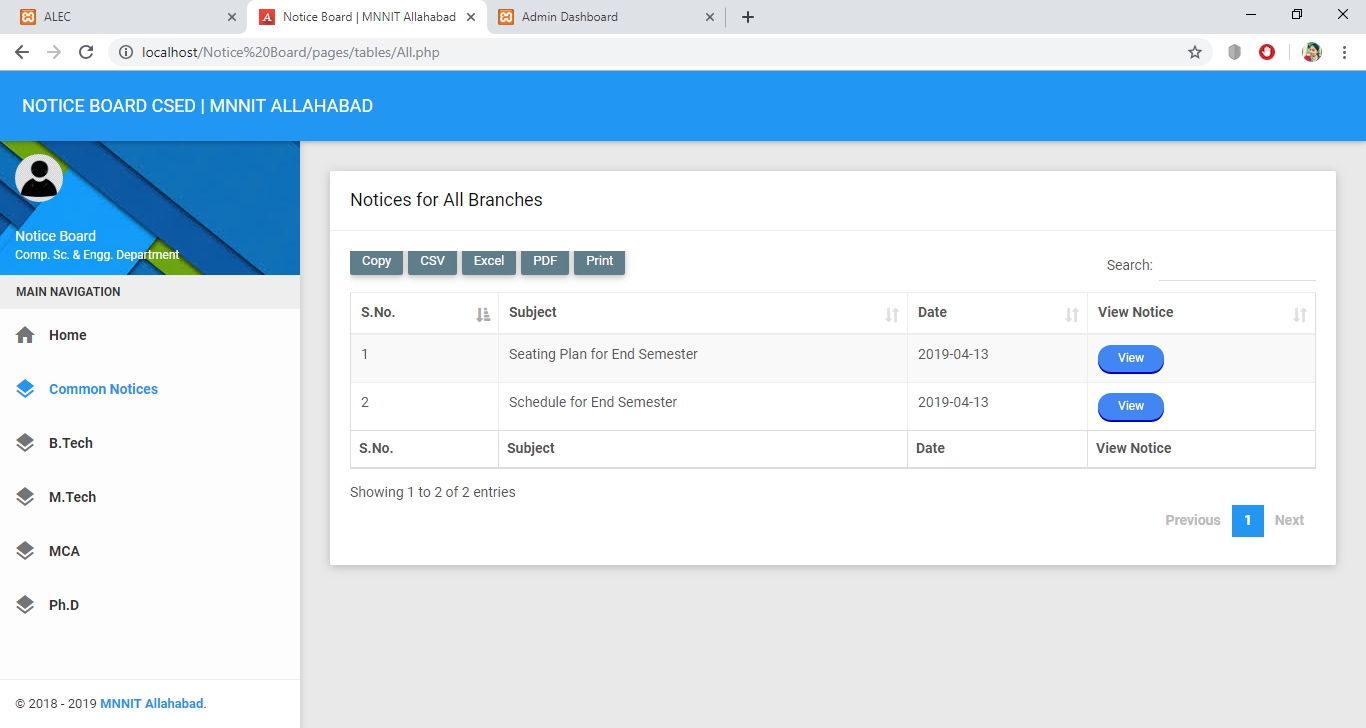
\includegraphics[width=\textwidth]{images/s5.png}
\begin{center}
Fig 9.5: \emph{Notices for all Branches}
\end{center}
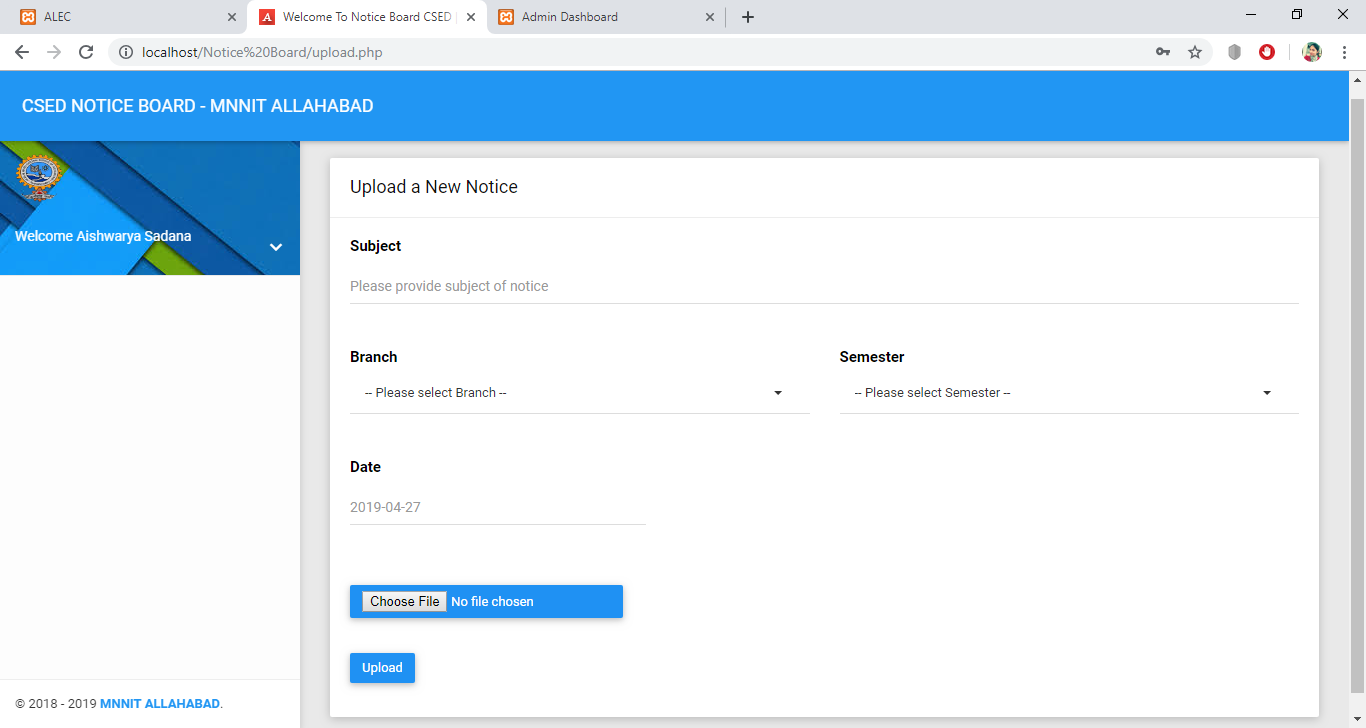
\includegraphics[width=\textwidth]{images/s6.png}
\begin{center}
Fig 9.6: \emph{Notice Board - Upload notice}
\end{center}
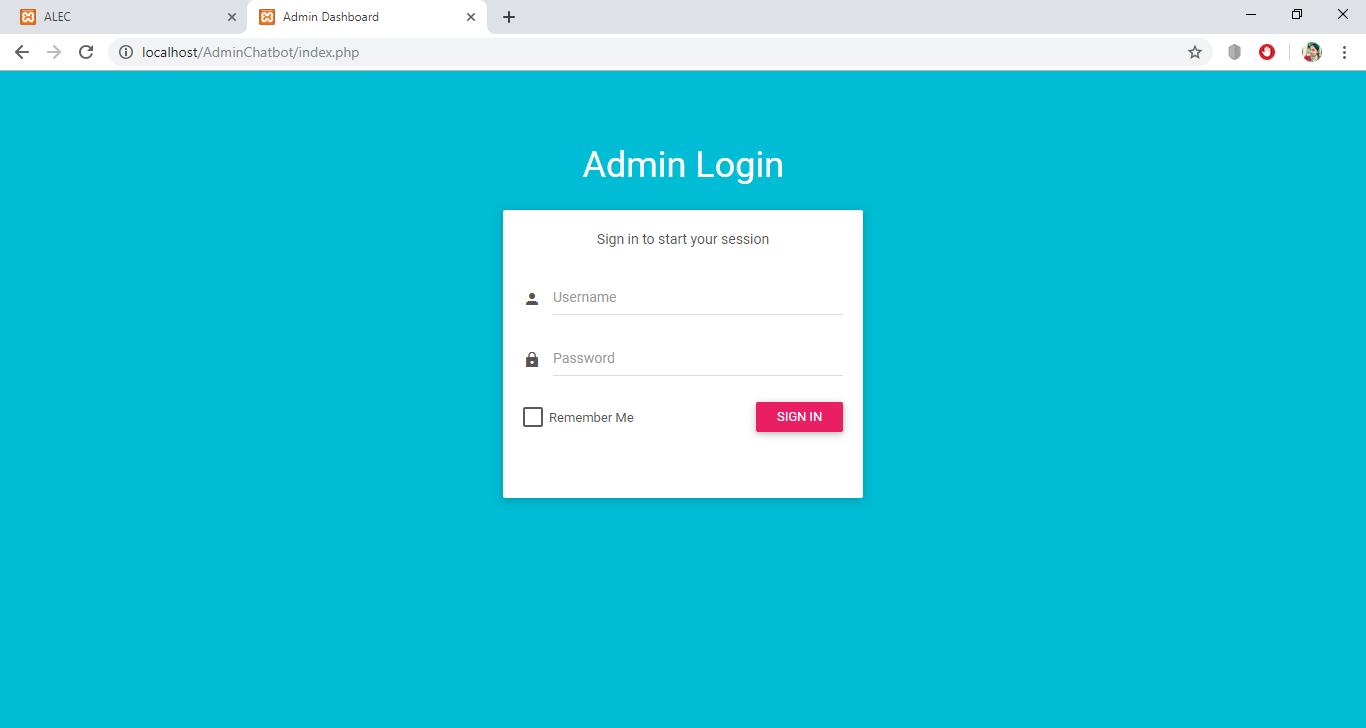
\includegraphics[width=\textwidth]{images/s7.png}
\begin{center}
Fig 9.7: \emph{Admin log in}\\
\end{center}
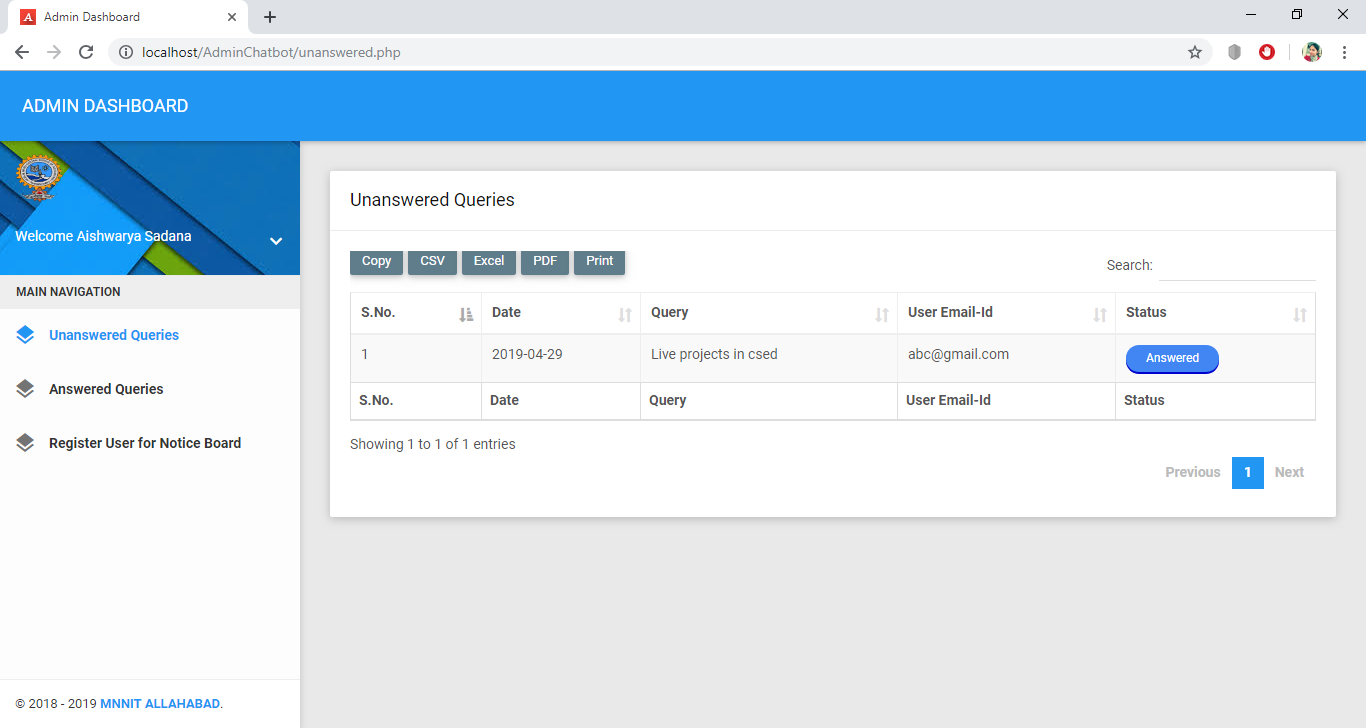
\includegraphics[width=\textwidth]{images/s8.png}
\begin{center}
Fig 9.8: \emph{Admin Dashboard - Unanswered Queries}\\
\end{center}
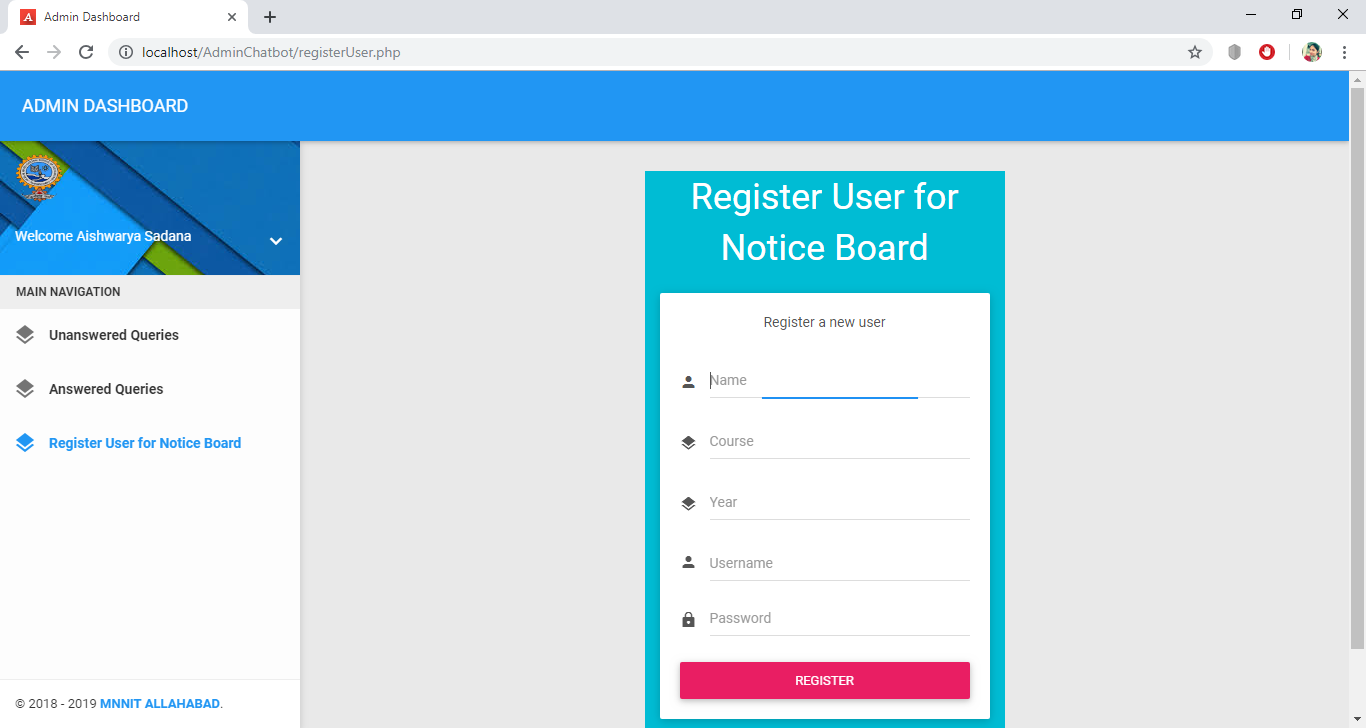
\includegraphics[width=\textwidth]{images/s9.png}
\begin{center}
Fig 9.9: \emph{Registration for notice board}\\
\end{center}


\user
\chapter{Conclusion and Future Work}
We now have a Web-app for our CSED Department that will be useful for the students to find answers to their queries. Though it may have a very limited number of features as of now, it can very easily be modified to add new features.\\\\
In future many other functionalities can be added to the portal like: 
\begin{itemize}
    \item If the answer is not proper or invalid, then as per user suggestion it can be modified by the admin
    \item Answers with the available options so that the user does not have to type his response.(predicted answers will be available to choose)
    \item Image and PDF in the answers
    \item Speech to text and text to speech feature.
    \item More effective notice board view.
    \item User login for more specific queries like assignment, marks or exam information.
    \item Publishing to social media platform.
\end{itemize}


\chapter{References}
\begin{enumerate}
	\item https://drive.google.com/file/d/0B-tCvLzyt01FYlQ2dVRBWEtTNkE/view
	\\(Research Paper referred)

	\item https://www.cleverbot.com/  \\(Normal user friendly chatbot)


	\item https://www.irctc.co.in/nget/  \\(A railway guide on IRCTC website)

	\item https://en.m.wikipedia.org/wiki/Xampp \\(Xampp server)

	\item https://chatterbot.readthedocs.io/en/stable/  \\(Python Chatterbot library)
\end{enumerate}




%\addcontentsline{toc}{chapter}{References}
\end{document}
